%----------------------------------------------------------------------------------------
%MAJOR CHAPTER 1
%----------------------------------------------------------------------------------------

\chapter{Part One}

%----------------------------------------------------------------------------------------

\section{Section 1}

\subsection{Sub-section 1}
\begin{wrapfigure}{R}{0.45\textwidth}
  \begin{center}
    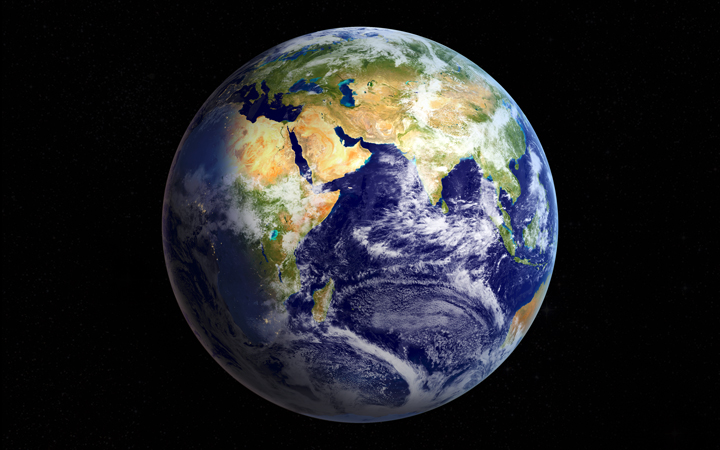
\includegraphics[width=0.45\textwidth]{earth}
  \end{center}
  \caption{Earth again}
\end{wrapfigure}

More about Earth

\subsection{Sub-section 2}
Earth earth earth

\subsubsection{Sub-sub-section 1}

A sub-sub-section for more details on earth.

% Example of a description (Used when describing a process step by step)
\begin{description}
\item[Big Bang] \hfill \\
Booooooom

\item[First Forms of life] \hfill \\
This time is called Archean.

\item[More Complex Life Forms] \hfill \\
Including forms of multicellular organisms etc.

\item[Dinosaurs and Humans] \hfill \\
Life expands\ldots
\end{description} 

% Example of Equation
\begin{equation}
\tan\alpha = \frac{x}{z} * \frac{180}{\pi} 
\end{equation}

